\documentclass{elsarticle}
\usepackage[utf8]{inputenc}

\usepackage{tikz-cd}
\usepackage{subfig}

\usepackage{graphicx}
\usepackage{caption}
\usepackage{xspace}
\usepackage{color}
\usepackage{subfig}
\usepackage{epstopdf}% To incorporate .eps illustrations using PDFLaTeX, etc.
\usepackage{comment}

\newcommand{\revOne}[1]{{\color{blue!80!black}#1}}
\newcommand{\revTwo}[1]{{\color{red!80!black}#1}}

%\usepackage[nolists,tablesfirst]{endfloat}% To `separate' figures and tables from text if required
\usepackage{amsmath,amssymb}
\usepackage{dsfont}
\usepackage{bm}
\usepackage{mathrsfs}
\usepackage{amsthm}
\usepackage{a4wide}

\usepackage{multirow}
\usepackage{diffcoeff}
\usepackage{arydshln,mathtools}% http://ctan.org/pkg/{arydshln,leftidx,mathtools}
\usepackage[most]{tcolorbox}


\usepackage[numbers]{natbib}% Citation support using natbib.sty
%\bibpunct[, ]{(}{)}{;}{a}{}{,}% Citation support using natbib.sty
%\renewcommand\bibfont{\fontsize{10}{12}\selectfont}% Bibliography support using natbib.sty
\bibliographystyle{unsrtnat}


\newtheorem{theorem}{Theorem}
\newtheorem{definition}{Definition}
\newtheorem{remark}{Remark}
\newtheorem{proposition}{Proposition}
\newtheorem{formula}{Formula}
\newtheorem{corollary}{Corollary}
\newtheorem{assumption}{Assumption}
\newtheorem{example}{Example}

\renewcommand\d{\ensuremath{\mathrm{d}}}


% inner products
\def\onedot{$\mathsurround0pt\ldotp$}
\def\cddot{% two dots stacked vertically
	\mathbin{\vcenter{\baselineskip.67ex
			\hbox{\onedot}\hbox{\onedot}}%
}}

\newcommand{\bbR}{\mathbb{R}}
\newcommand{\bbF}{\mathbb{F}}
\newcommand{\bbA}{\mathbb{A}}
\newcommand{\bbB}{\mathbb{B}}
\newcommand{\bbS}{\mathbb{S}}

\DeclareMathOperator{\tr}{tr}

\newcommand*{\dual}[1]{\ensuremath{\widehat{#1}}}
\newcommand*{\norm}[1]{\ensuremath{\left\|#1\right\|}}
\newcommand{\where}{\qquad \text{where} \qquad}

\newcommand{\inpr}[3][]{\ensuremath{\langle #2, \, #3 \rangle_{#1}}}

\newcommand{\dualpr}[3][]{\ensuremath{\langle #2 \, \vert #3 \rangle_{#1}}}


\newcommand{\pder}[2]{\ensuremath{\partial_{#2} #1}}
\newcommand{\dder}[2]{\ensuremath{\delta_{#2} #1}}

\DeclareMathOperator*{\grad}{grad}
\DeclareMathOperator*{\Grad}{Grad}
\DeclareMathOperator*{\Div}{Div}
\renewcommand{\div}{\operatorname{div}}
\DeclareMathOperator*{\Hess}{Hess}
\DeclareMathOperator*{\curl}{curl}

\newcommand{\secref}[1]{\S\ref{#1}}
\newcommand{\energy}[1]{\frac{1}{2} \int_{\Omega} \left\{ #1 \right\} \d\Omega}
\newcommand{\crmat}[1]{\ensuremath{\left[#1\right]_\times}}
\newcommand{\fenics}{\textsc{FEniCS}\xspace}
\newcommand{\firedrake}{\textsc{Firedrake}\xspace}




\journal{ArXiv}

\graphicspath{{./images/}}

\begin{document}

\section{Introduction}

\subsection{Algebraic topology}



\begin{definition}[$k$-simplex]
Consider $k+1$, $k\le n$ distinct points $(\mathbf{p}_0, \dots, \mathbf{p}_k)$ in $\bbR^n$, that are affinely independent (i.e. they span a $k$-plane). A $k$ simplex $\sigma_k$ is defined as
the convex hull of the points $\mathbf{p}_i$
\begin{equation}
    \sigma_k :=
     \left\{\sum_{i=0}^k \theta_i \mathbf{p}_i \Bigg| \;  \sum_{i=0}^k \theta_i = 1, \quad \theta_i\ge 0 \right\}.
\end{equation}
or the following more succinct notation will be used: $\sigma_k = [\mathbf{p}_0, \dots, \mathbf{p}_k]$.
\end{definition}

\begin{definition}[Simplicial complex]
A simplicial complex $\mathcal{S}$ is a finite set  of simplices in $\bbR^n$ such that whenever a simplex belongs to $\mathcal{S}$, each of its faces also belongs to $\mathcal{S}$, and if $f$ and $g$ are two simplices in $\mathcal{S}$, then their intersection $f \cap g$ is either empty or a common face. \\

\noindent Given a  simplicial complex $\mathcal{S}$ in $\bbR^n$, $\Delta_k(\mathcal{S})$ denotes its set of simplices of dimension $k$:
$\mathcal{S}=\cup_{k=[0, \dots, n]} \Delta_k(\mathcal{S})$.
\end{definition}

  

\begin{definition}[Simplicial $k$-chain]
A $k$-chain is a formal linear combination of $k$-simplices $\sigma_k^i
\in \Delta_k(\mathcal{S}):$
\begin{equation}
c_k := \sum_{i \in I, \; \sigma_k^i
\in \Delta_k(\mathcal{S})} a_i \sigma_k^i
\end{equation}
where $a_i \in \mathbb{R}$ and $I$ is a generic index set. The set of all
$k$-chains is denoted by $C_k$. By construction, this set has the structure of a vector space spanned by all $k$-simplices.
\end{definition}

\begin{definition}[Boundary of $k$-simplices and chains]\label{def:bd_chain}
The boundary $\partial_{k-1}$ of a $k$-simplex $\sigma_k$ is  defined as the $k-1$ chain given by
\begin{equation}
    \partial_{k-1}\sigma_k = \partial_{k-1} [\mathbf{p}_0, \dots, \mathbf{p}_k] := \sum_{j=0}^k (-1)^j [\mathbf{p}_0, \dots, \widetilde{\mathbf{p}}_{j},  \dots,\mathbf{p}_k].
\end{equation}
where $k=1, \dots, n$ and $\widetilde{\mathbf{p}}_{i}$ means that that vertex is omitted. The boundary of a chain is defined by linearity
\begin{equation}
    \partial_{k-1} c_k = \sum_{i \in I} a_i \partial_{k-1} \sigma_k^i
\end{equation}
\end{definition}
From Definition \ref{def:bd_chain}, it follows $\partial_{k-1}\partial_k=0$. Associated to a simplicial complex, one has what is called
the simplicial chain complex (cf. Fig. \ref{fig:cd_cochain}).
Particularly important is the dual space $C^k$ to the vector space of chains~$C_k$. The elements of $C^k$ are called $k$-cochains. The duality pairing between $k$-chains and $k$-cochains is denoted by $\dualpr[C_k]{\cdot}{\cdot}$.
\begin{definition}[Coboundary operator]
The adjoint of the boundary operator, the coboundary operator $\partial^k : C^k \rightarrow C^{k+1}$, is expressed by the relation
\begin{equation}
    \dualpr[C_k]{a^k}{\partial_{k} c_{k+1}} = \dualpr[C_{k+1}]{\partial^k a^k}{c_{k+1}}, \qquad a^k \in C^k, \; c_{k+1} \in C_{k+1},
\end{equation}
so that $\partial^k = \partial_{k}'$. Using as basis of $C^{k+1}$ the canonical dual basis to the basis for $C_{k+1}$, it is immediate to see that the algebraic realization of these operators satisfy $\bm{\partial}^k = \bm{\partial}_{k+1}^\top$.
\end{definition}
From this definition, it follows that $\partial^{k+1}\partial^{k}$. The dual complex to the chain complex is the cochain complex (cf. Fig. \ref{fig:cd_cochain}). Using as basis  for $C_k$ the $\sigma_k^i$ simplexes $\forall i=0, \dots, \# \Delta_k(\mathcal{S})$ (symbol $\#$ denotes the cardinality of a set), an algebraic realization of cochains is obtained in terms of coefficients vectors by means of the canonical dual basis $\dual{\sigma}_k^i$ \cite{bochev2006,hiemstra2014}. The
canonical dual basis leads to $\dualpr{\dual{\sigma}_k^i}{\sigma_k^j}=\delta_{ij}$ where $\delta_{ij}$ denotes the Kronecker delta symbol. The de Rham map provides a natural way to convert a differential form into a cochain as it will be shown for the Whitney forms.

\begin{figure}[h]
\centering
\begin{tikzcd}
C_0 & C_1 \arrow[l, swap, "\partial_0"] & \dots \arrow[l, swap, "\partial_1"]  & C_k \arrow[l, swap, "\partial_{k-1}"] & \dots \arrow[l, swap, "\partial_k"] & C_{n-1} \arrow[l, swap, "\partial_{n-2}"] & C_n \arrow[l, swap, "\partial_{n-1}"] \\
C^0 \arrow[r, "\partial^0"] & C^1 \arrow[r, "\partial^1"] & \dots \arrow[r, "\partial^{k-1}"] & C^k \arrow[r, "\partial^k"] & \dots \arrow[r, "\partial^{n-2}"] & C^{n-1} \arrow[r, "\partial^{n-1}"] & C^n
\end{tikzcd} 
\caption{The duality between the chain complex (top) and cochain complex (bottom).}
\label{fig:cd_cochain}
\end{figure}



\subsection{Finite element differential forms}

In this section, finite element differential forms are briefly recalled. This is precisely treated in the context of Exterior Calculus with what is known as Finite Elements Exterior Calculus (FEEC)  framework \cite{arnold2006acta,arnold2018finite}. \\

Let $\mathcal{T}_h$ be a shape regular triangulation of $M \subset \bbR^n$, i.e. the simplicial complex corresponding to the computational mesh. The mesh is composed by triangles if $n=2$ or tetrahedra if $n=3$. The generic element is denoted by $T$. Here, we focus on the trimmed polynomial family $\mathcal{P}^-_s\Omega^k(\mathcal{T}_h)$. As shown in \cite{arnold2006acta}, the dimension of the trimmed polynomial space for a generic element 
$T$ of the mesh is given by the following expression \begin{equation*}
\mathrm{dim}\; \mathcal{P}^-_s\Omega^k(T)=\begin{pmatrix}
s+n \\
s+k
\end{pmatrix}
\begin{pmatrix}
s+k-1 \\
k
\end{pmatrix}
\end{equation*}

In the lowest order case $s=1$, the second term is identically one, leading to 
\begin{equation*}
    \mathrm{dim}\; \mathcal{P}^-_1\Omega^k(T)=\begin{pmatrix}
1+n \\
1+k
\end{pmatrix}.
\end{equation*}
Considering for example $n=3$, $T$ is a tetrahedron (composed of $4$ vertices, $6$ edges $4$ faces and $1$ volume), and the spaces of differential forms have dimensions
\begin{equation*}
   \mathrm{dim}\; \mathcal{P}^-_1\Omega^0(T)= 4, \qquad \mathrm{dim}\; \mathcal{P}^-_1\Omega^1(T)= 6, \qquad \mathcal{P}^-_1\Omega^2(T)= 4, \qquad \mathcal{P}^-_1\Omega^3(T)= 1,
\end{equation*}
which shows that there is exactly one degree of freedom for each $k$-simplex (cf. Fig. \ref{fig:whitneyforms}). The same applies in any spatial dimension $n$. The lowest order space $\mathcal{P}^-_1\Omega^k(T)$ corresponds to the so-called $k$-Whitney forms. For them there is an isomorphism between simplicial cochain complex and the Whitney forms complex, given by the de Rham map. 

\begin{figure}[tbh]%
\centering
\subfloat[][$\mathcal{P}^-_1\Omega^0(T)$]{%
	\label{fig:whitney0}%
	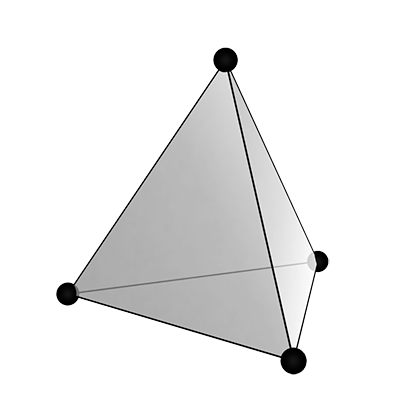
\includegraphics[width=0.23\columnwidth]{P1_tetrahedron.png}}%
\hspace{8pt}%
\subfloat[][$\mathcal{P}^-_1\Omega^1(T)$]{%
	\label{fig:whitney1}%
	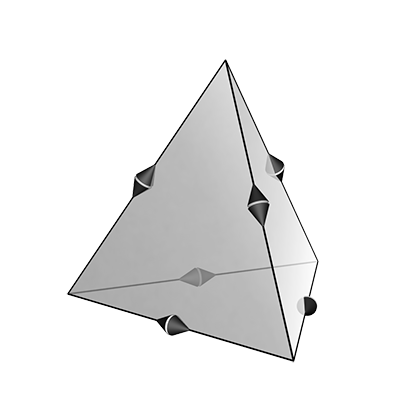
\includegraphics[width=0.23\columnwidth]{N1e1_tetrahedron.png}}%
\hspace{8pt}%
\subfloat[][$\mathcal{P}^-_1\Omega^2(T)$]{%
	\label{fig:whitney2}%
	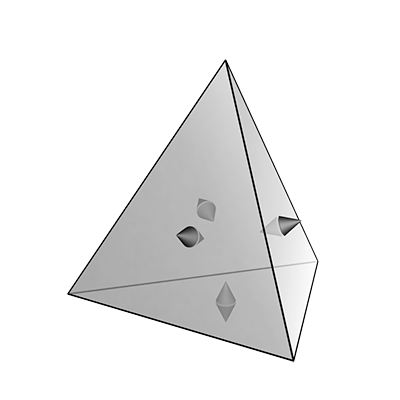
\includegraphics[width=0.23\columnwidth]{N1f1_tetrahedron.png}}
	\hspace{8pt}%
\subfloat[][$\mathcal{P}^-_1\Omega^3(T)$]{%
	\label{fig:whitney3}%
	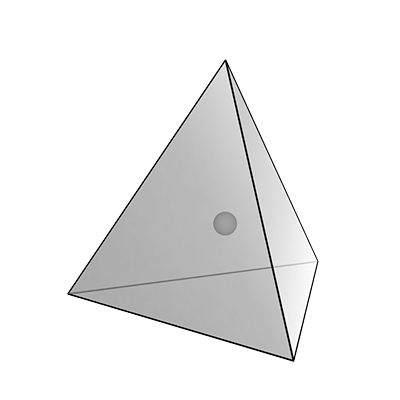
\includegraphics[width=0.23\columnwidth]{dP0_tetrahedron.png}}
\caption{The Whitney forms degrees of freedom in three dimensions (taken from \cite[Page 91]{arnold2018finite})}%
\label{fig:whitneyforms}%
\end{figure}

It is possible to generalise the Whitney forms as first order finite elements to the case of higher order $s>1$. This is be done by introducing  conforming finite element families arising from the Finite Element Exterior Calculus framework. As we have seen previously, for a $s$ order finite element method, we can associate to each element $\mathrm{dim}( \mathcal{P}^-_s\Omega^k(T))$ basis forms. Higher order cases of the trimmed polynomial spaces are constructed by defining extra degrees of freedom (reported in \cite[Eq. 5.2]{arnold2006acta}) in the finite element. The general construction of the
polynomial spaces of differential forms is given in \cite{arnold2006acta,arnold2018finite}. 


\subsubsection{Whitney forms}
The Whitney forms are the 
oldest finite elements for differential forms, as they were introduced by Whitney in the fifties \cite{whitney1957}. Whitney forms are constructed by composing the de Rham map and the Whitney interpolation. The de Rham map represents a reduction, since it converts a form into a cochain. The interpolation instead reconstructs a differential form from a cochain.  The space of $k-$cochains over the mesh $\mathcal{T}_h$ is denoted by $C^k(\mathcal{T}_h)$ and the set of $k-$simplexes by $\Delta_k(\mathcal{T}_h)$.

\begin{definition}[de Rham map]
Given a $k$-simplex $\sigma_k^j \in \Delta_k(\mathcal{T}_h)$, the de Rham map is defined as
\begin{equation*}
    \mathcal{R}^k:
\Omega^k(M) \rightarrow C^k(\mathcal{T}_h) ; \qquad \omega^k \mapsto  a^k:=
\sum_{j=1}^{\# \Delta_k(\mathcal{T}_h)}
\dual{\sigma}_k^j
 \int_{\sigma_k^j} \tr_{\sigma_k^j} \omega^k
\end{equation*}
where $\tr_{\sigma_k^j}:=\iota_k^*$ is the pullback of the inclusion map $\iota_k: \sigma_k^j \rightarrow \mathcal{T}_h$
and $\dual{\sigma}_k^j \in C^k$ is the dual basis of $\sigma_k^j \in C_k$.
\end{definition}

\begin{definition}[Whitney interpolation]
Let $\lambda_i:\bbR^n \rightarrow \bbR$
be the barycentric function associated to the vertex $\mathbf{p}_i$ in the 
simplicial complex $\mathcal{T}_h$ representing the computational mesh
(i.e. the unique linear function satisfying $\lambda_i(\mathbf{p}_j) = \delta_{ij}$). \\
The Whitney basis function $w_j^k$ associated to the simplex $\sigma_k^j = [\mathbf{p}_0, \dots, \mathbf{p}_k]$ is computed as
\begin{equation}
    w^k_j := k! \sum_{i=0}^k (-1)^i \lambda_i \d\lambda_0 \wedge \dots \widetilde{\d\lambda}_i \wedge \dots \wedge \d\lambda_k,
\end{equation}
where $\widetilde{\d\lambda}_i$ indicates that $\d\lambda_i$ is omitted. The Whitney interpolation $\mathcal{I}^k$ is the map
\begin{equation*}
    \mathcal{I}^k:
  C^k(\mathcal{T}_h) \rightarrow \Omega^k(M) ; \qquad 
    a^k \mapsto \omega^k_h:= \sum_{j=1}^{\# \Delta_k(\mathcal{T}_h)}  \dualpr[C_k]{a^k}{\sigma_k^j} w^k_j.
\end{equation*}
\end{definition}
The Whitney interpolation is a conforming map. This means that its range is a subspace of the Sobolev space $H\Omega^k(M)$, i.e. $\text{ran}(\mathcal{I}^k)=\text{span}(w^k_1, \hdots, w^k_{\#\Delta_k(\mathcal{T}_h)})
\subset H\Omega^k(M)$. A proof of this statement can be found in \cite[Theorem 4.4.]{gillette2011stability}. The range of the Whitney interpolation corresponds to the lowest order trimmed polynomial space $\text{range}(\mathcal{I}^k) = \mathcal{P}^{-}_1\Omega^k(\mathcal{T}_h)$. The following commutativity properties are of fundamental importance for discretization. We consider forms belonging to the domain of the exterior derivative 
%the 
space~$H\Omega^k(M)$. 
\begin{theorem}\cite[Section IV.27]{whitney1957}\label{th:cd_RI}
The following commutativity relations hold for the de Rham map and Whitney interpolation 

\begin{enumerate}
\item $\mathcal{R}^{k+1} \d^k = \partial^k \mathcal{R}^k;$
\item $\d^k \mathcal{I}^k = \mathcal{I}^{k+1} \partial^k$ (Conforming operator).
\end{enumerate}
\begin{figure}[h]
\centering
\begin{tikzcd}
H\Omega^k(M) \arrow[r, "\d^k"] \arrow[d, "\mathcal{R}^k"]
& H\Omega^{k+1}(M) \arrow[d, "\mathcal{R}^{k+1}"] \\
C^k(\mathcal{T}_h) \arrow[r, "\partial^k"]
& C^{k+1}(\mathcal{T}_h)
\end{tikzcd} \hspace{1cm}
\begin{tikzcd}
C^k(\mathcal{T}_h) \arrow[r, "\partial^k"] \arrow[d, "\mathcal{I}^k"]
& C^{k+1}(\mathcal{T}_h) \arrow[d, "\mathcal{I}^{k+1}"] \\
\mathcal{P}^{-}_1\Omega^k(\mathcal{T}_h) \arrow[r, "\d^k"] 
& \mathcal{P}^{-}_1\Omega^{k+1}(\mathcal{T}_h)  
\end{tikzcd} 
\caption{Commuting diagrams for the de Rham map (left) and  Whitney interpolation (right).}
\label{fig:cd_RI}
\end{figure}

\end{theorem}

Given a generic $k$-form $\omega$, one can consider its projection onto the Whitney forms  by composing the de Rham map   and the Whitney interpolation~$\mathcal{I}^k \circ \mathcal{R}^k$~\cite{bochev2006}
\begin{equation}
\Pi_{1, h}^{-, k}:H\Omega^k(M) \rightarrow 
 \mathcal{P}^{-}_1\Omega^{k}(\mathcal{T}_h) 
; \qquad \omega^k \mapsto \omega_h^k:=(\mathcal{I}^k \circ \mathcal{R}^k )(\omega)
\end{equation}
$\Pi^{-, k}_{1, h}$ corresponds to a linear projector from the functional space $H\Omega^k(M) $ to the (finite-dimensional) functional subspace formed by the image of the Whitney forms. The error in the projection represents the error due to the interpolation and can be expressed by means of an $L^2$ inner product:
\begin{equation}\label{eq:L2err}
   \text{Err}(\omega):
H\Omega^k(M) \rightarrow \mathbb{R} ; \qquad 
\omega \mapsto \inpr[M]{\omega-\Pi_{1, h}^{-, k}(\omega)}{\omega-\Pi_{1, h}^{-, k}(\omega)} 
\end{equation}

An immediate corollary of Theorem~\ref{th:cd_RI} is that the commutativity property extends to the projector 
\begin{equation*}
\d^k \Pi_{1, h}^k = \Pi_{1, h}^{k+1}\d^k.    
\end{equation*}
This property, that goes under the name of {\it cochain property} \cite{arnold2018finite}, is fundamental and common to all the different families of finite element differential forms. It basically represents the compatibility and preservation of the differential structure in the subspace of the projection, it basically shows that $\Pi_{1, h}^{-, k}$ is a structure preserving map with the structure being the topological one represented by $\d^k$. It is important to realise that the particularity of the Whitney forms resides in the fact that the commutativity property holds at the level of both the interpolation and the reduction map. This is due to the fact that Whitney forms are highly geometrical, since they associate to each $k$-dimensional subsimplex only one degree of freedom as illustrated before.

\subsubsection{Higher order forms}
The general construction of higher order finite element differential forms is here reported. The discussion follows \cite{wu2021hodgewave}. \\


Denote $\mathcal{P}_s(\bbR^n)$ as the space of polynomials of degree at most $s$ on an $n$-dimensional Euclidian space, and $\mathcal{H}_s(\bbR^n)$ as the space of homogeneous polynomial functions of degree $s$. Homogeneous polynomials are polynomials for which the sum of the exponents of each summing term has the same value $s$ resulting in a homogeneous function of degree $s$.

Spaces of $s$-th order polynomial differential $k-$forms, indicated as $\mathcal{P}_s\Omega^k(\bbR^n)$, and their homogeneous subclass, indicated as $\mathcal{H}_s \Omega^k(\bbR^n)$, can be defined by using the corresponding polynomials as the coefficients. Given a point $\xi \in \bbR^n$, one can treat $\xi$ as a vector in the tangential space $T_\xi\bbR^n$, and define the Koszul operator $\kappa : \Omega^k (\bbR^n) \rightarrow \Omega^{k - 1} (\bbR^n)$ 
\begin{equation}
    (\kappa\omega)_\xi(v_1, v_2, . . . , v_{k - 1}) = \omega_\xi(\xi, v_1, v_2, \dots, v_{k - 1}).
\end{equation}
The Koszul operator $\kappa$ satisfies \cite[Thm. 3.1.]{arnold2006acta}
$$\kappa\d + \d\kappa = (k + s)\mathrm{Id}.$$
By means of the Koszul operator, the space of homogeneous polynomial $\mathcal{H}_s\Omega^k(\bbR^n)$, is written as the direct sum
\begin{equation}
    \mathcal{H}_s\Omega^k(\bbR^n) = \kappa \mathcal{H}_{s - 1}\Omega^{k+1}(\bbR^n) \oplus \d\mathcal{H}_{s+1}\Omega^{k - 1}(\bbR^n).
\end{equation}

Given this decomposition, the trimmed space of polynomial $k$-form is defined as
\begin{equation}
    \mathcal{P}^-_s\Omega^k(\bbR^n)  = \mathcal{P}_{s - 1}\Omega^k(\bbR^n) + \kappa \mathcal{H}_{s - 1}\Omega^{k+1}(\bbR^n).
\end{equation}
The spaces of $k$-forms on the computational mesh $\mathcal{P}_s\Omega^k(\mathcal{T}_h)$ (resp. $\mathcal{P}^-_s\Omega^k(\mathcal{T}_h)$ are obtained by restricting the forms $\mathcal{P}_s\Omega^k(\bbR^n)$ (resp. $\mathcal{P}_s^-\Omega^k(\bbR^n)$), to the elements $T$ ($n$-simplexes) of the computational mesh~$\mathcal{T}_h$. The following finite element spaces are then obtained
\begin{equation}
\begin{aligned}
    \mathcal{P}_s\Omega^k(\mathcal{T}_h) &= \{\omega \in H\Omega^k(M) |\quad \omega|_T \in \mathcal{P}_s\Omega^k(T) \quad \forall T \in \mathcal{T}_h\}, \\
\mathcal{P}_s^-\Omega^k(\mathcal{T}_h) &= \{\omega \in H\Omega^k(M) |\quad \omega|_T \in \mathcal{P}_s^-\Omega^k(T) \quad \forall T \in \mathcal{T}_h\}.
\end{aligned}
\end{equation}
The Whitney forms correspond to the case $\mathcal{P}_1^-\Omega^k(\mathcal{T}_h) = \mathcal{P}_0\Omega^k(\mathcal{T}_h) + \kappa \mathcal{P}_0\Omega^k(\mathcal{T}_h)$. The degrees of freedom for the space $\mathcal{P}_s\Omega^k(T)$ are given by
\begin{equation}\label{eq:dof_P}
    \omega \in \mathcal{P}_s\Omega^k(T) \rightarrow \int_{\sigma_j} (\tr_{\sigma_j} \omega) \wedge \mu, \qquad \mu \in \mathcal{P}^-_{s+k-j}\Omega^{j-k}(\sigma_j), \quad \sigma_j \in \Delta_j(\mathcal{T}_h), \quad j \ge k.
\end{equation}
For the space $\mathcal{P}_s^-\Omega^k(T)$ the degrees of freedom are obtained via
\begin{equation}\label{eq:dof_P-}
    \omega \in \mathcal{P}_s^-\Omega^k(T) \rightarrow \int_{\sigma_j} (\tr_{\sigma_j} \omega) \wedge \mu, \qquad \mu \in \mathcal{P}_{s+k-j-1}\Omega^{j-k}(\sigma_J), \quad \sigma_j \in \Delta_j(\mathcal{T}_h), \quad j \ge k.
\end{equation}
These polynomial spaces form a subcomplex of the de Rham complex.
\begin{theorem}{\cite[Lemma 3.8]{arnold2006acta}}\label{th:fe_subcomplex}
The complexes $(\mathcal{P}_s\Omega^k(\mathcal{T}_h), \d), \; (\mathcal{P}_s^-\Omega^k(\mathcal{T}_h), \d)$ forms a subcomplex of $(H\Omega^k(M), \d)$
\begin{equation*}
    \d\mathcal{P}_s\Omega^k(\mathcal{T}_h) \subset \mathcal{P}_{s-1}\Omega^{k+1}(\mathcal{T}_h), \qquad \d\mathcal{P}^-_s\Omega^k(\mathcal{T}_h) \subset \mathcal{P}^-_s\Omega^{k+1}(\mathcal{T}_h),
\end{equation*}
or graphically
\begin{equation*}
\begin{aligned}
    0\longrightarrow \mathcal{P}_s\Omega^0(\mathcal{T}_h) \overset{\d}{\longrightarrow} \mathcal{P}_{s - 1}\Omega^1(\mathcal{T}_h) \overset{\d}{\longrightarrow} \dots \overset{\d}{\longrightarrow} \mathcal{P}_{s - n}\Omega^n(\mathcal{T}_h) \longrightarrow 0.\\
    0 \longrightarrow \mathcal{P}^-_s \Omega^0(\mathcal{T}_h) \overset{\d}{\longrightarrow} \mathcal{P}^-_s \Omega^1(\mathcal{T}_h) \overset{\d}{\longrightarrow} \dots
\overset{\d}{\longrightarrow} \mathcal{P}^-_s \Omega^n(\mathcal{T}_h) \longrightarrow 0.
\end{aligned}
\end{equation*}
\end{theorem}
One fundamental property of the finite element differential forms is the fact that their projector commute with the exterior derivative (this property is also called cochain property). 
\begin{theorem}\cite[Thm. 5.2.]{arnold2006acta}
Denoting by  $\Pi_{s, h}^{k}$ (resp. $\Pi_{s, h}^{-, k}$) the projector onto the space $\mathcal{P}_s\Omega^k(\mathcal{T}_h)$ (resp. $\mathcal{P}_s^-\Omega^k(\mathcal{T}_h)$), one has 
\begin{equation}
    \d \Pi_{s, h}^{k} \omega^k = \Pi_{s-1, h}^{k+1} \d \omega^k, \qquad \d \Pi_{s, k}^{-, k} \omega^k = \Pi_{s, h}^{-, k+1} \d \omega^k, \quad \omega^k \in \Omega^k(M).
\end{equation}

\begin{figure}[h]
\centering
\begin{tikzcd}
H\Omega^k(M) \arrow[r, "\d^k"] \arrow[d, "\Pi_{s, h}^{k}"]
& H\Omega^{k+1}(M) \arrow[d, "\Pi_{s-1, h}^{k+1}"] \\
\mathcal{P}_s\Omega^k(\mathcal{T}_h) \arrow[r, "\d^k"]
& \mathcal{P}_s\Omega^k(\mathcal{T}_h)
\end{tikzcd} \hspace{1cm}
\begin{tikzcd}
H\Omega^k(M) \arrow[r, "\d^k"] \arrow[d, "\Pi_{s, h}^{-, k}"]
& H\Omega^{k+1}(M) \arrow[d, "\Pi_{s, h}^{-, k+1}"] \\
\mathcal{P}_s^-\Omega^k(\mathcal{T}_h) \arrow[r, "\d^k"]
& \mathcal{P}_s^-\Omega^k(\mathcal{T}_h)
\end{tikzcd}  
\caption{Commuting diagrams for the finite element differential forms projectors.}
\label{fig:cd_FEDF}
\end{figure}
\end{theorem}




\bibliography{biblio_revision}


\end{document}